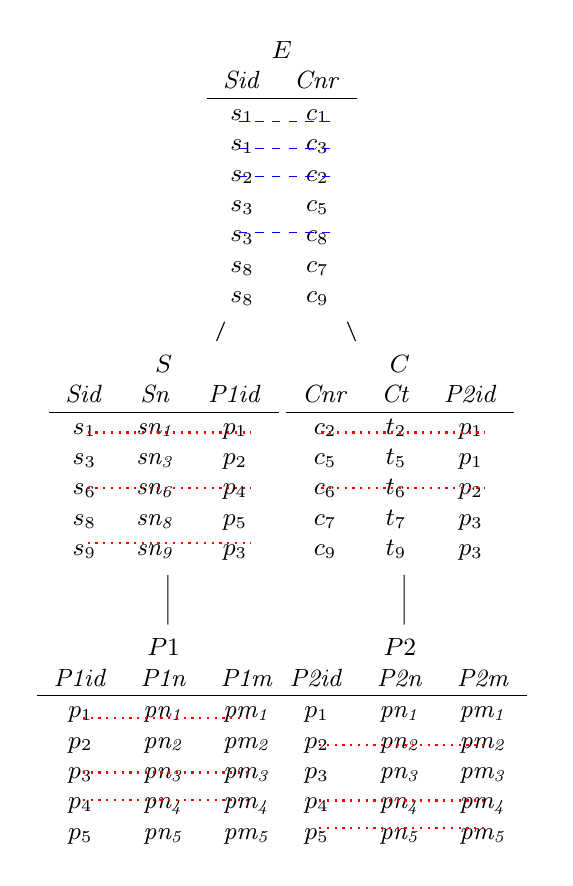
\begin{tikzpicture}[scale=0.6]
    \node	(5)	at	(-2.5,-8)	[align=center]	{
		\small
		\begin{tabular}{ccc}
			\multicolumn{3}{c}{$P1$}\\
			$\mathit{P1id}$ & $\mathit{P1n}$ & $\mathit{P1m}$ \\
			\hline
			$p_1$ & $\mathit{pn_1}$ & $\mathit{pm_1}$ \\
			$p_2$ & $\mathit{pn_2}$ & $\mathit{pm_2}$ \\
			$p_3$ & $\mathit{pn_3}$ & $\mathit{pm_3}$ \\
			$p_4$ & $\mathit{pn_4}$ & $\mathit{pm_4}$ \\
			$p_5$ & $\mathit{pn_5}$ & $\mathit{pm_5}$ \\
		\end{tabular}
	};
	\draw[red,dotted,thick] (-4.3,-7.5) -- (-.7,-7.5);
	\draw[red,dotted,thick] (-4.3,-8.66) -- (-.7,-8.66);
	\draw[red,dotted,thick] (-4.3,-9.24) -- (-.7,-9.24);
	\node	(4)	at	(2.5,-8)	[align=center]	{
		\small
		\begin{tabular}{ccc}
			\multicolumn{3}{c}{$P2$}\\
			$\mathit{P2id}$ & $\mathit{P2n}$ & $\mathit{P2m}$ \\
			\hline
			$p_1$ & $\mathit{pn_1}$ & $\mathit{pm_1}$ \\
			$p_2$ & $\mathit{pn_2}$ & $\mathit{pm_2}$ \\
			$p_3$ & $\mathit{pn_3}$ & $\mathit{pm_3}$ \\
			$p_4$ & $\mathit{pn_4}$ & $\mathit{pm_4}$ \\
			$p_5$ & $\mathit{pn_5}$ & $\mathit{pm_5}$ \\
		\end{tabular}
	};
	\draw[red,dotted,thick] (.7,-8.08) -- (4.3,-8.08);
	\draw[red,dotted,thick] (.7,-9.25) -- (4.3,-9.25);
	\draw[red,dotted,thick] (.7,-9.83) -- (4.3,-9.83);
	\node	(3)	at	(2.5,-2)	[align=center]	{
		\small
		\begin{tabular}{ccc}
			\multicolumn{3}{c}{$C$}\\
			$\mathit{Cnr}$ & $\mathit{Ct}$ & $\mathit{P2id}$ \\
			\hline
			$c_2$ & $t_2$ & $p_1$ \\
			$c_5$ & $t_5$ & $p_1$ \\
			$c_6$ & $t_6$ & $p_2$ \\
			$c_7$ & $t_7$ & $p_3$ \\
			$c_9$ & $t_9$ & $p_3$ \\
		\end{tabular}
	}
		edge(4);
	\draw[red,dotted,thick] (.75,-1.46) -- (4.2,-1.46);
	\draw[red,dotted,thick] (.75,-2.63) -- (4.2,-2.63);
	\node	(2)	at	(-2.5,-2)	[align=center] {
		\small
		\begin{tabular}{ccc}
			\multicolumn{3}{c}{$S$}\\
			$\mathit{Sid}$ & $\mathit{Sn}$ & $\mathit{P1id}$ \\
			\hline
			$s_1$ & $\mathit{sn_1}$ & $p_1$ \\
		    $s_3$ & $\mathit{sn_3}$ & $p_2$ \\
		    $s_6$ & $\mathit{sn_6}$ & $p_4$ \\
		    $s_8$ & $\mathit{sn_8}$ & $p_5$ \\
		    $s_9$ & $\mathit{sn_9}$ & $p_3$ \\
		\end{tabular}
	}
	    edge(5);
	\draw[red,dotted,thick] (-4.2,-1.46) -- (-.75,-1.46);
	\draw[red,dotted,thick] (-4.2,-2.63) -- (-.75,-2.63);
	\draw[red,dotted,thick] (-4.2,-3.8) -- (-.75,-3.8);
	\node	(1)	at	(0,4)		[align=center]	{
		\small
		\begin{tabular}{cc}
			\multicolumn{2}{c}{$E$}\\
			$\mathit{Sid}$ & $\mathit{Cnr}$ \\
			\hline
			$s_1$ & $c_1$ \\
			$s_1$ & $c_3$ \\
			$s_2$ & $c_2$ \\
			$s_3$ & $c_5$ \\
			$s_3$ & $c_8$ \\
			$s_8$ & $c_7$ \\
			$s_8$ & $c_9$ \\
		\end{tabular}
	}
		edge(2)
		edge(3);
	\draw[blue,dashed] (-1,5.12) -- (1,5.12);
	\draw[blue,dashed] (-1,4.54) -- (1,4.54);
	\draw[blue,dashed] (-1,3.95) -- (1,3.95);
	\draw[blue,dashed] (-1,2.78) -- (1,2.78);
\end{tikzpicture}